% !TeX spellcheck = en_US

\chapter{Experiments}
The goal of this project was not only to build a control system that provides both scalability and availability, but also to compare it to the current solution by Siemens Windpower. 
In order to evaluate the system, we have created the experiments in the following sections.

Every experiment is done using 3 computers connected using a 1Gbit ethernet router with IGMP support.
The experiments are run on 3 laptops, with one being used to capture test data and the other 2 optionally running a number of turbines controllers to generate traffic.
All test are run with CPU utilization on average below 90\%, this is done to keep performance consistent.
The specification of the hardware used for testing can be found in \cref{appendix:HardwareSpecification}

\section{Scalability Experiments}
Scalability is by Bondi\cite{Bondi:2000:CSI:350391.350432} defined as the systems ability to accommodate an increasing number of elements or objects, to process growing volumes of work gracefully, and/or to be susceptible to enlargement. 

The experiments below are engineered to show how the number of turbines affect performance characteristics parameters, the test are done with 2, 21, 41, 61, 81 and 101 simulated turbine controllers. Besides turbines we are also going to modify ''Data Wait Time Frame'' witch is a constant that defines the time a turbine controller will wait for new updates before considering the other turbine controller offline and unavailable.

%Theses characteristics are depended on some experiment configuration here are the parameters that we are going to adjust during our experiments:

%\begin{description}
%	\item [Data Wait time frame] The time the systems waits for other systems to send data and to receive this data.
%	\item [Turbine offline delay] The time a turbine controller will wait for new updates before considering the other turbine controller offline and unavailable.
%\end{description}

\subsection{Cycle time}
This parameter is measured by every node and transmitted to every node, this is bundled together with the data packets as described in \cref{sec:algoDecen,sec:algoCen}.


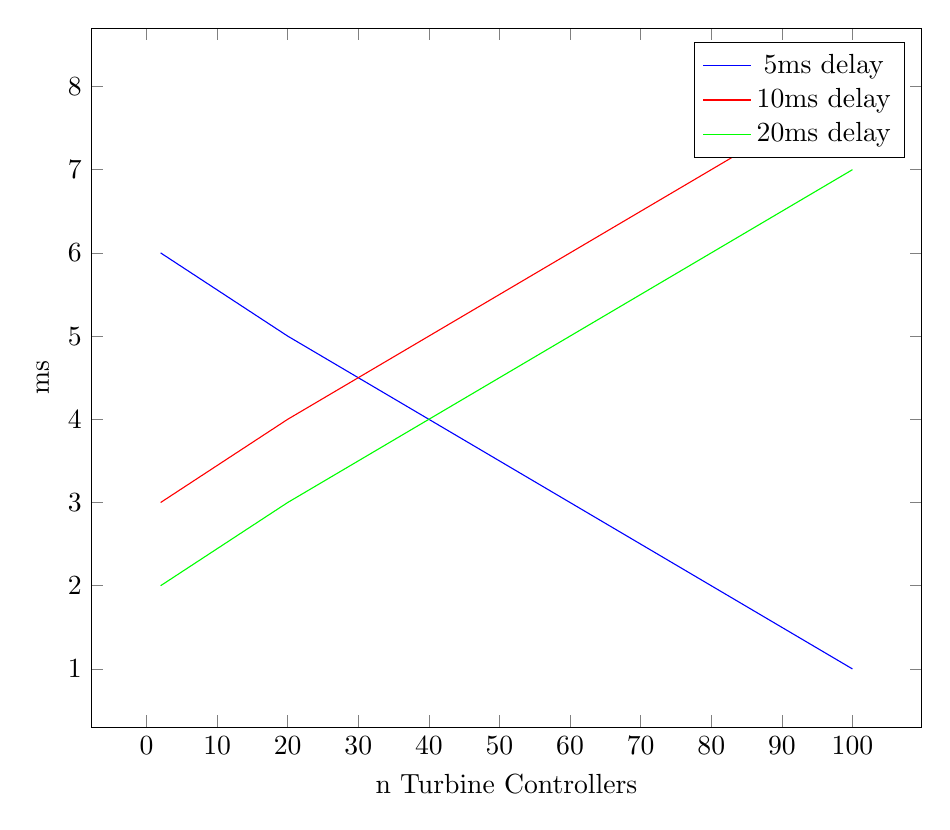
\begin{tikzpicture}
\begin{axis}[
width=\textwidth,
%ymax=0.5,
xlabel=n Turbine Controllers,
ylabel=ms]
\addplot[blue!20!blue] coordinates {
	(2 ,6)
	(20 ,5)
	(40 ,4)
	(60 ,3)
	(80 ,2)
	(100 ,1)
		};
\addplot[red!20!red] coordinates {
	(2 , 3)
	(20 ,4)
	(40 ,5)
	(60 ,6)
	(80 ,7)
	(100,8)	
	};
\addplot[green!20!green] coordinates {
		(2 , 2)
		(20 ,3)
		(40 ,4)
		(60 ,5)
		(80 ,6)
		(100,7)	
	};
\legend{5ms delay,10ms delay,20ms delay}
\end{axis}
\end{tikzpicture}


\subsection{Cache misses}
This information is also added to the packets every turbine is sending, this parameter tells how many turbine controllers where unable to respond in the given data wait time frame. This is meant to give a real life clue to how increased network traffic results in data not being recived before its deadline. The deadline is the ''Data Wait Time Frame'' value.

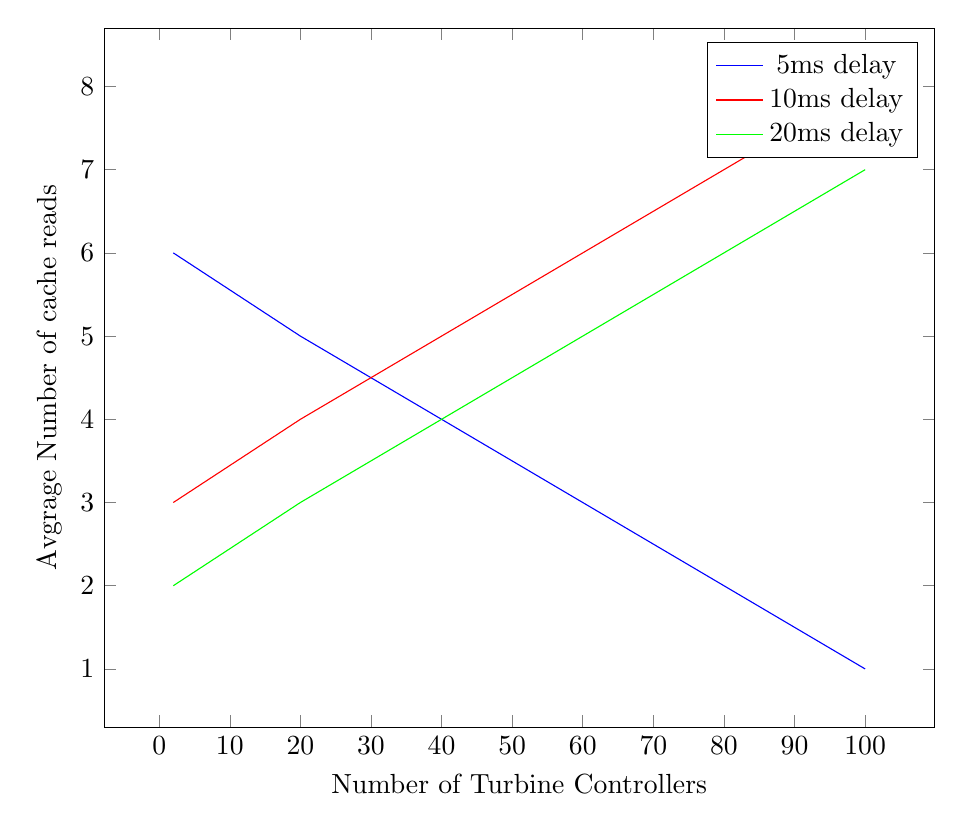
\begin{tikzpicture}
\begin{axis}[
width=\textwidth,
%ymax=0.5,
xlabel=Number of Turbine Controllers,
ylabel=Avgrage Number of cache reads]
\addplot[blue!20!blue] coordinates {
		(2 ,6)
		(20 ,5)
		(40 ,4)
		(60 ,3)
		(80 ,2)
		(100 ,1)
	};
\addplot[red!20!red] coordinates {
		(2 , 3)
		(20 ,4)
		(40 ,5)
		(60 ,6)
		(80 ,7)
		(100,8)	
	};
\addplot[green!20!green] coordinates {
		(2 , 2)
		(20 ,3)
		(40 ,4)
		(60 ,5)
		(80 ,6)
		(100,7)	
	};
\legend{5ms delay,10ms delay,20ms delay}
\end{axis}
\end{tikzpicture}



\subsection{System resources}
\paragraph{Memory consumption} The memory footprint of the application is measured locally on the machine running the test instance, no memory data is collected form the machine running multiple instances. The test system is expected to be running only one instance, therefore measuring memory consumption on machines running multiple instances is therefor not done.	
	
\paragraph{Network utilization} Is also measured locally on the machine running the test instance, it is further described in the test cases.

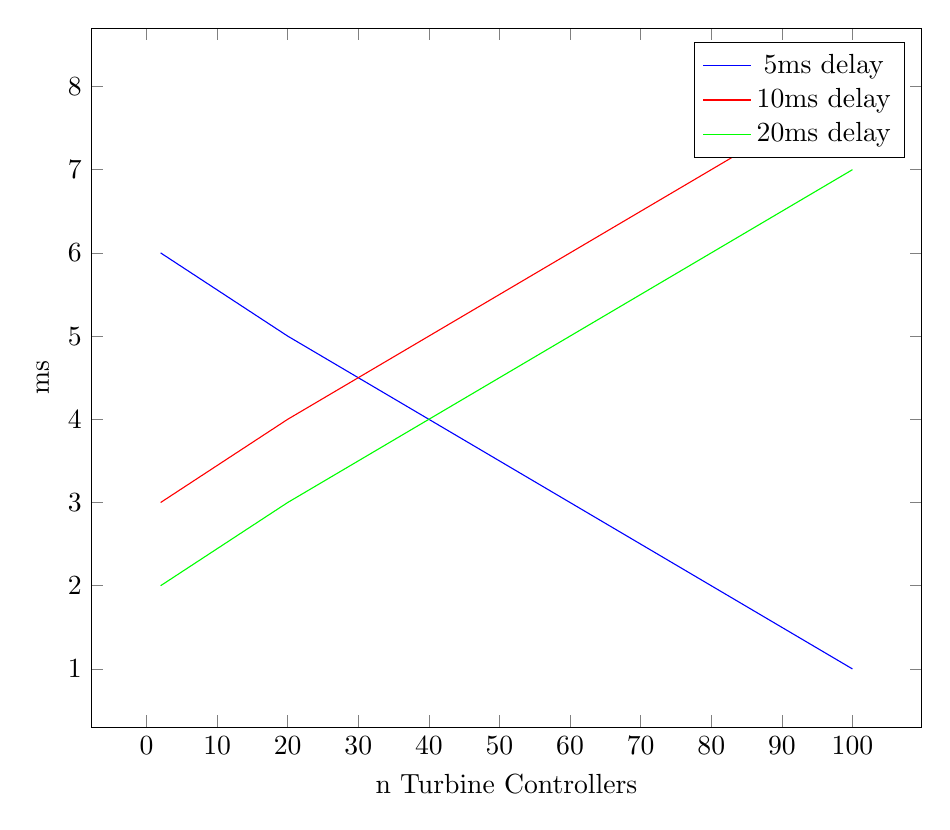
\begin{tikzpicture}
\begin{axis}[
width=\textwidth,
%ymax=0.5,
xlabel=n Turbine Controllers,
ylabel=ms]
\addplot[blue!20!blue] coordinates {
	(2 ,6)
	(20 ,5)
	(40 ,4)
	(60 ,3)
	(80 ,2)
	(100 ,1)
		};
\addplot[red!20!red] coordinates {
	(2 , 3)
	(20 ,4)
	(40 ,5)
	(60 ,6)
	(80 ,7)
	(100,8)	
	};
\addplot[green!20!green] coordinates {
		(2 , 2)
		(20 ,3)
		(40 ,4)
		(60 ,5)
		(80 ,6)
		(100,7)	
	};
\legend{5ms delay,10ms delay,20ms delay}
\end{axis}
\end{tikzpicture}


	
\section{Availability Experiments}

Randomly kill client, plot a few seconds of data around the event.



%\begin{description}
%	\item [CPU load] (Using THIS API, THIS COMMAND LINE TOOL)
%	\item [Cycle time] This parameter is measured by every node and transmitted to every node, this is bundled together with the data packets as described in \cref{sec:algoDecen,sec:algoCen}.
%	\item [Number of cache misses] This information is also added to the packets every turbine is sending, this parameter tells how many turbine controllers where unable to respond in the given data wait time frame. 
%	\item [Memory consumption] The memory footprint of the application is measured locally on the machine running the test instance, no memory data is collected form the machine running multiple instances. The test system is expected to be running only one instance, therefore measuring memory consumption on machines running multiple instances is therefor not done.
%	\item [Network utilization] Is also measured locally on the machine running the test instance, it is further described in the test cases.
%\end{description}
